\chapter{Literatür Taraması}

Derin öğrenme son yıllarda popüler bir araştırma konusu olmuştur. Bununla birlikte gelişen yüksek 
hızlı hesaplamalı ekran kartları ile büyük boyutlu görüntülerin de çalışmaları artmıştır.\\

Adaptive spatial-spectral feature learning network(ASSFLN) yöntemi olarak bir yöntem. İlk olarak görüntüyü parçalara bölme işlemi yapıldı ve daha sonra merkez-komşluk spectrum çiftleri oluşturulmuştur. Bu işlem adımlarından sonra vektör olarak çıkan sonuçlar 2B olarak birleştirdi. Daha sonra bunları ESA ve SAE(Stack Autoencoder) ile birlikte kullanmış. ESA işleminden sonra softmax normalizasyon ile ağırlık öğrenme ağı oluşturmuş. Daha sonra öğrenilen her bir ağırlığın özelliğini çıkarıp bunları  stack autoencoder a vermiş. Bu işlemin sonunda çıktıyı MLR( multinomial logistic regression) katmanına aktarıp sınıflandırmayı bu aşamada yapmıştır \cite{li2019adaptive}. Şekil 3.1'de anlatılan modelin görsel hali verilmiştir. \\

\begin{figure}[!ht]
  \centering
  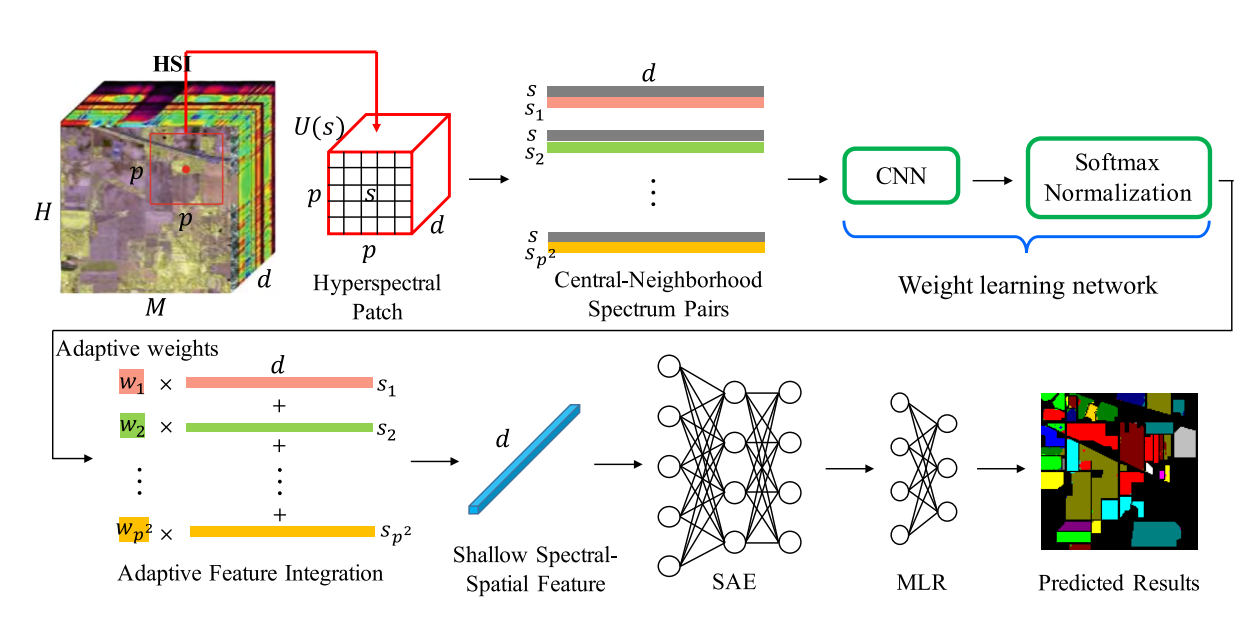
\includegraphics[width=1\textwidth]{Figures/assfln13.png}
  \caption{ASSFLN modelinin genel olarak çalışma şekli }
\end{figure}

\newpage
Bir başka bir yöntem ise. İlki hyperspectral görüntülerden tek tek pikselleri alıyor. Bu işlem için flat diye bir yöntem uyguluyor. Burada bahsedilen flat işlemi bu piksellerin birleştirmesini ifade ediyor. Sonra çıkardığı her bir pikselleri  başka bir yöntem olan pixel gömme olarak birleşitiryor.  Sonra BERT ismi verilen bir sıralı ağa veriyor. Bu işlemin ardından çıktıları tam-bağlı ağa verip burada eğittikten sonra sınıflandırma işlemi yapıyor \cite{he2019hsi}. Şekil 3.2'de anlatılan modelin görsel hali verilmiştir. \\

\begin{figure}[!ht]
  \centering
  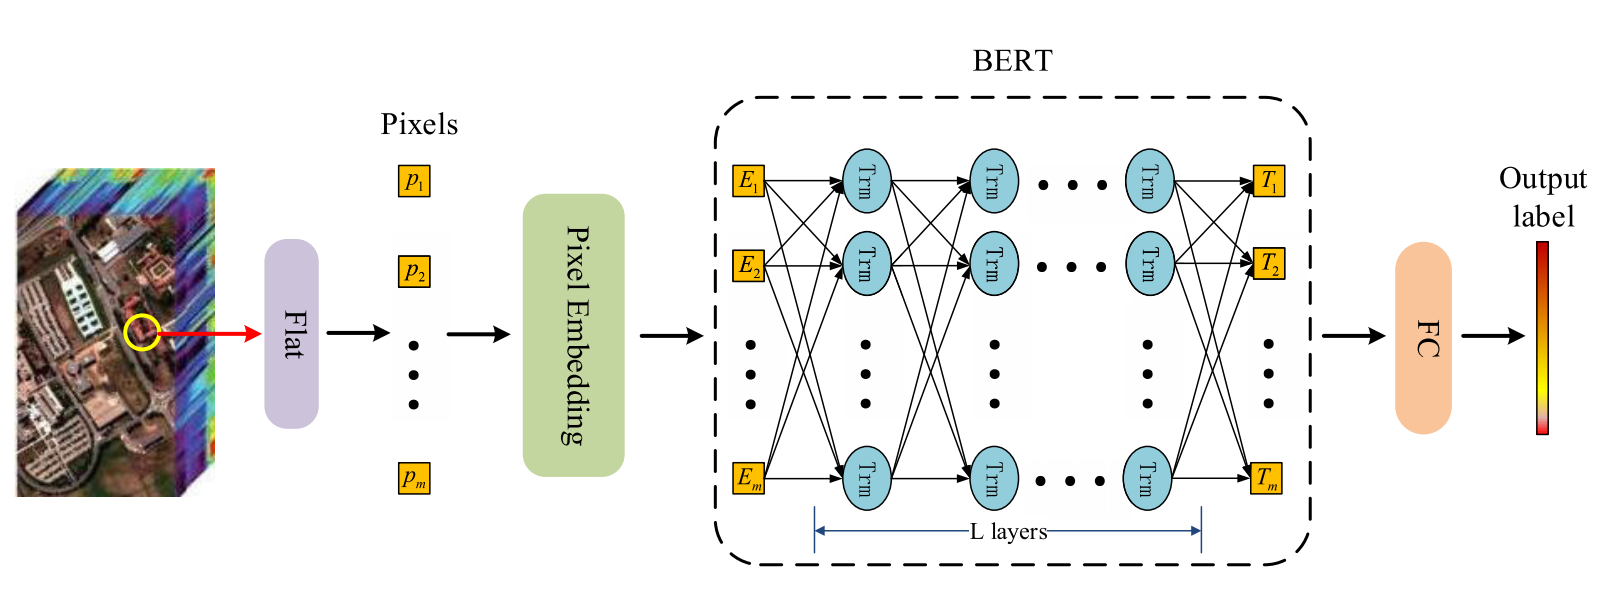
\includegraphics[width=1\textwidth]{Figures/bert14.png}
  \caption{BERT modelinin genel olarak çalışma şekli }
\end{figure}

\newpage
Yöntem temel olarak sınıflardan eşit örnek alınarak farklı ESA mimarilarinden oluşturulmuştur. Bu ESA mimarileri şunlardır; 3B-ESA, 2B-ESA,  D-3B ESA, D-2B ESA, D-Res-2B ESA, D-Res-3B-ESA mimarileri ile traning yapılıyor. Bunların çıktıları her birini bir vektör olarak hesaplıyor ve etkiket verileri ile arasında euclide uzaklığını hesaplıyor ve ardınan yitim( loss) fonksiyonuna veriyor. Danışmanlı özellikler(Supervised feature) çıkarıp Sinir Ağı(Neural Network) sınıflandırıcı ile sınıflandırıyor. Test amaçlı SVM ve bunun türevleri olan sınıflandırıca kulanılıyor fakat en iyi sonucu NN veriyor. Res olarak bahsedilen mimari son zamanlarda derin öğrenmede kullanılan residual olarak adı geçen yapıdır. Bir önceki ağdan gelen çıkıtıyı o anki ağdan çıkan çıktı ile toplama işlemi olarak kısaca anlatabiliriz \cite{roy2019hybridsn}. Şekil 3.3'de anlatılan modelin görsel hali verilmiştir. \\


\begin{figure}[!ht]
  \centering
  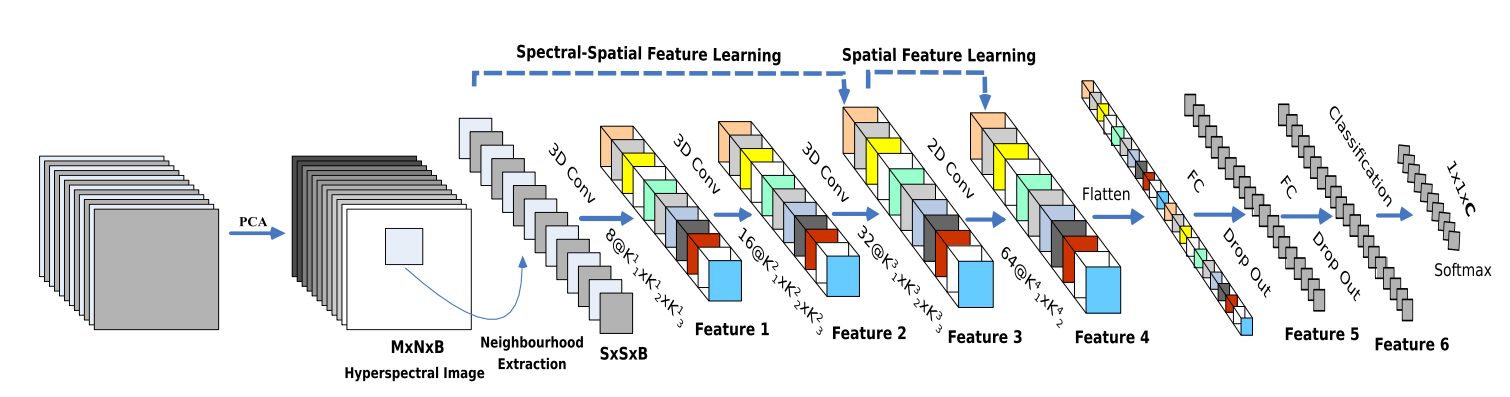
\includegraphics[width=1\textwidth]{Figures/hybrdidSN15.png}
  \caption{HybridSN modelinin genel olarak çalışma şekli }
\end{figure}

\newpage
Görüntü patchlere bölündükten sonra conv uygulanıp ardından pre-activation residual attention network yapılmıştır. Bunun amacı gradiant vanishing/explosing gibi problemleri önlemek ve sınıflandırma performansını arttırmak için yapmıştır. Sınıflandırma aşamasından önceği katman da ise global average pooling (GAP) kullanılmıştır ve daha sonra klasik sinir ağına verilip sınıflandırma yapılmıştır. Kayıp fonksiyonu olarak cross entropy loss kullanılmıştır. Residual blokları için relu kullanılmıştır. Son katman çıkışı olarak da sigmoid kullanılmıştır \cite{gao2019hyperspectral}.Şekil 3.4'de anlatılan modelin görsel hali verilmiştir. \\

\begin{figure}[!ht]
  \centering
  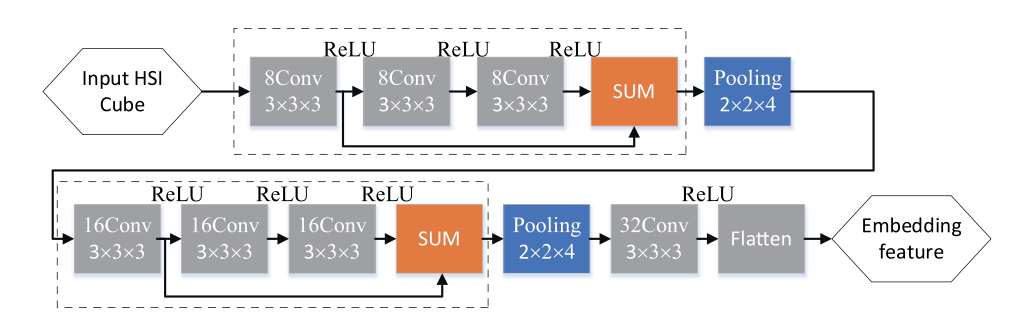
\includegraphics[width=1\textwidth]{Figures/gao16.png}
  \caption{GAO modelinin genel olarak çalışma şekli }
\end{figure}
\newpage
Giriş görüntüleri patchlere bölünüyor preporcessing olarak. Daha sonra spectral feature extraction için Evrişim 1*1 ve ReLU uygulanıyor.Bu işlemin ardından çoklu spectral-spatial feature learning işlemleri yapılıyor. Yanda görsel olarak verildiği gibi. Bu aşamadan sonra concatenated yapılıp feature fusion yaparak devam ediyor. Çıkış katmanında ise softmax kullanıyor \cite{bai2019ssdc}. Şekil 3.5'de anlatılan modelin görsel hali verilmiştir. \\

\begin{figure}[!ht]
  \centering
  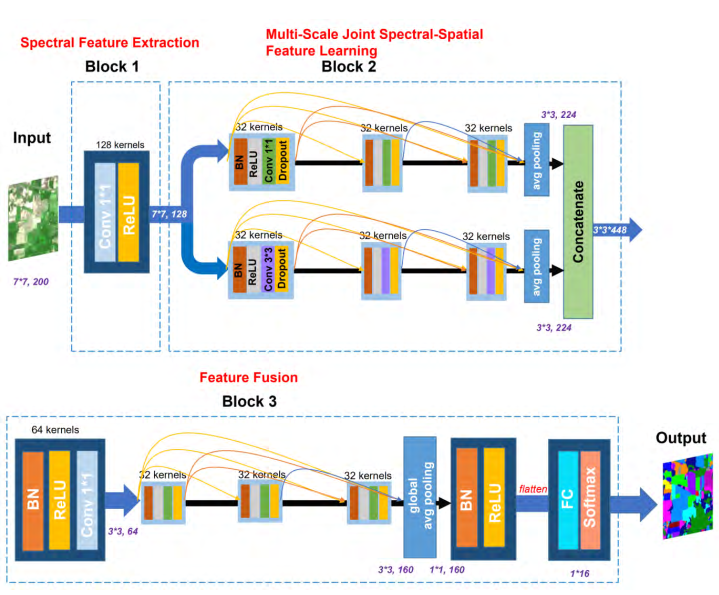
\includegraphics[width=1\textwidth]{Figures/ssfl17.png}
  \caption{SSDC-DenseNet modelinin genel olarak çalışma şekli }
\end{figure}

\newpage
İki aşamalı bir modeldir. İlk aşamada samples extranctions , yani örneklerden özellik çıkarma işlemi yapılıyor. Sonra 3B-SRNet  ağı ile özellik çıkarımı ve sınıflandırma işlemi yapıyor \cite{jiang2019hyperspectral}. Şekil 3.6'de anlatılan modelin görsel hali verilmiştir. \\

\begin{figure}[!ht]
  \centering
  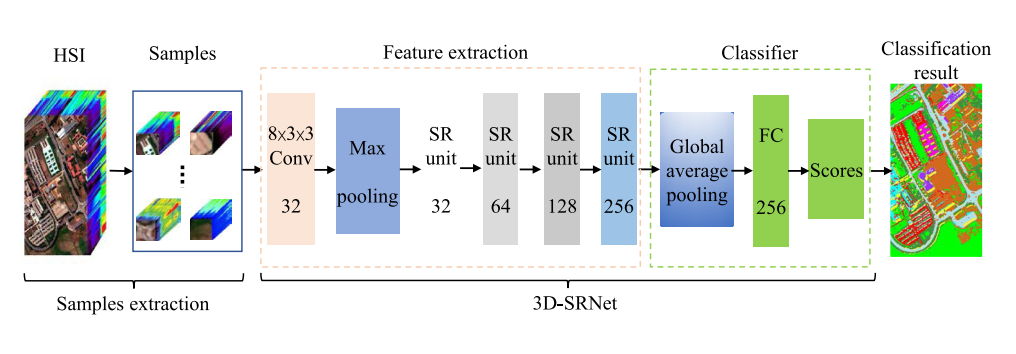
\includegraphics[width=1\textwidth]{Figures/3Dsrnet18.png}
  \caption{3D-SRNet modelinin genel olarak çalışma şekli }
\end{figure}















